\section{Knowledge Representation in the Semantic Web \textcolor{red}{-- By 19/1}}
\label{sec:chp2_semweb}

\textit{This section describes some background knowledge about concepts that play a relevant role in knowledge representation on the web. First we look into RDF, used for representing knowledge graphs on the web. Then we go over different approaches to reify knowledge in RDF, useful for representing additional information beyond triple paradigm. ??}

\subsection{Resource Description Framework (RDF)}

The Resource Description Framework (RDF)~\parencite{rdf} is a standard model for data interchange on the web. Its basic unit are triples: two concepts linked by a relationship. These triples are represented in the form of $<$ \textit{s,p,o} $>$, where \textit{s} is the subject, \textit{p} is the predicate and \textit{o} the object. This model relies on the use on the linking structure of the Web, using IRIs to identify uniquely every resource and relationship. 

\cref{lst:chp2_rdf-example} presents an example of an RDF graph composed of a set of triples about pole vault records, which is also visually depicted in \cref{fig:chp2_rdf-example}. In total there are four triples. They all share the same subject, which is a resource uniquely identified by the IRI $<$\texttt{http://example.com/athlete/1}$>$. Likewise, all predicates in the triples are also defined by an IRI, e.g. $<$\texttt{http://example.com/ns\#name}$>$. The first triple (Line 5) defines that the subject is an instance of the class \texttt{ex:Athlete} with the predicate \texttt{rdf:type}. The rest of the triples define attributes to this instance with name (\texttt{ex:name}) and height of a jump (\texttt{ex:mark}). The objects of both triples are literals, that may be strings ("Yelena Isinbayeva", Line 6) or typed literals ("5.06"\scalebox{.8}{\textsuperscript{$\wedge\wedge$}}\texttt{xsd:float}, Line 7). Type literals refer to data values attached with a tag that represents their data type.

\begin{minipage}{\textwidth}
\begin{captionedlisting}{lst:chp2_rdf-example}{Example of RDF graph.}
\centering
{\begin{lstlisting}[language=r2rml]
@prefix rdf: <http://www.w3.org/1999/02/22-rdf-syntax-ns#>.
@prefix xsd: <http://www.w3.org/2001/XMLSchema#>.
@prefix ex: <http://example.com/ns#>.

<http://example.com/athlete/1> rdf:type ex:Athlete .
<http://example.com/athlete/1> ex:name "Yelena Isinbayeva" .
<http://example.com/athlete/1> ex:mark "5.06"^^xsd:float .
\end{lstlisting}}
\end{captionedlisting}
\end{minipage}

There are different syntaxes to serialize RDF graphs. RDF/XML\footnote{\url{https://www.w3.org/TR/rdf-syntax-grammar}} was the first to be proposed, and relies on XML. Notation3 (N3)\footnote{\url{https://www.w3.org/TeamSubmission/n3/}} was developed as a human readable syntax, but its use is not common. Instead, the N-Triples\footnote{\url{https://www.w3.org/TR/n-triples}} and Turtle\footnote{\url{https://www.w3.org/TR/turtle}} serializations, subsets of N3, are more widely used. JSON-LD\footnote{\url{https://www.w3.org/TR/json-ld11}} was developed for programming environments, as it comprised in JSON documents. Lastly, RDFa\footnote{\url{https://www.w3.org/TR/rdfa-primer}} extends HTML to markup structured content in webpages, with the objective of improving the results retrieved by search engines. 



\begin{figure*}[t]
\centering
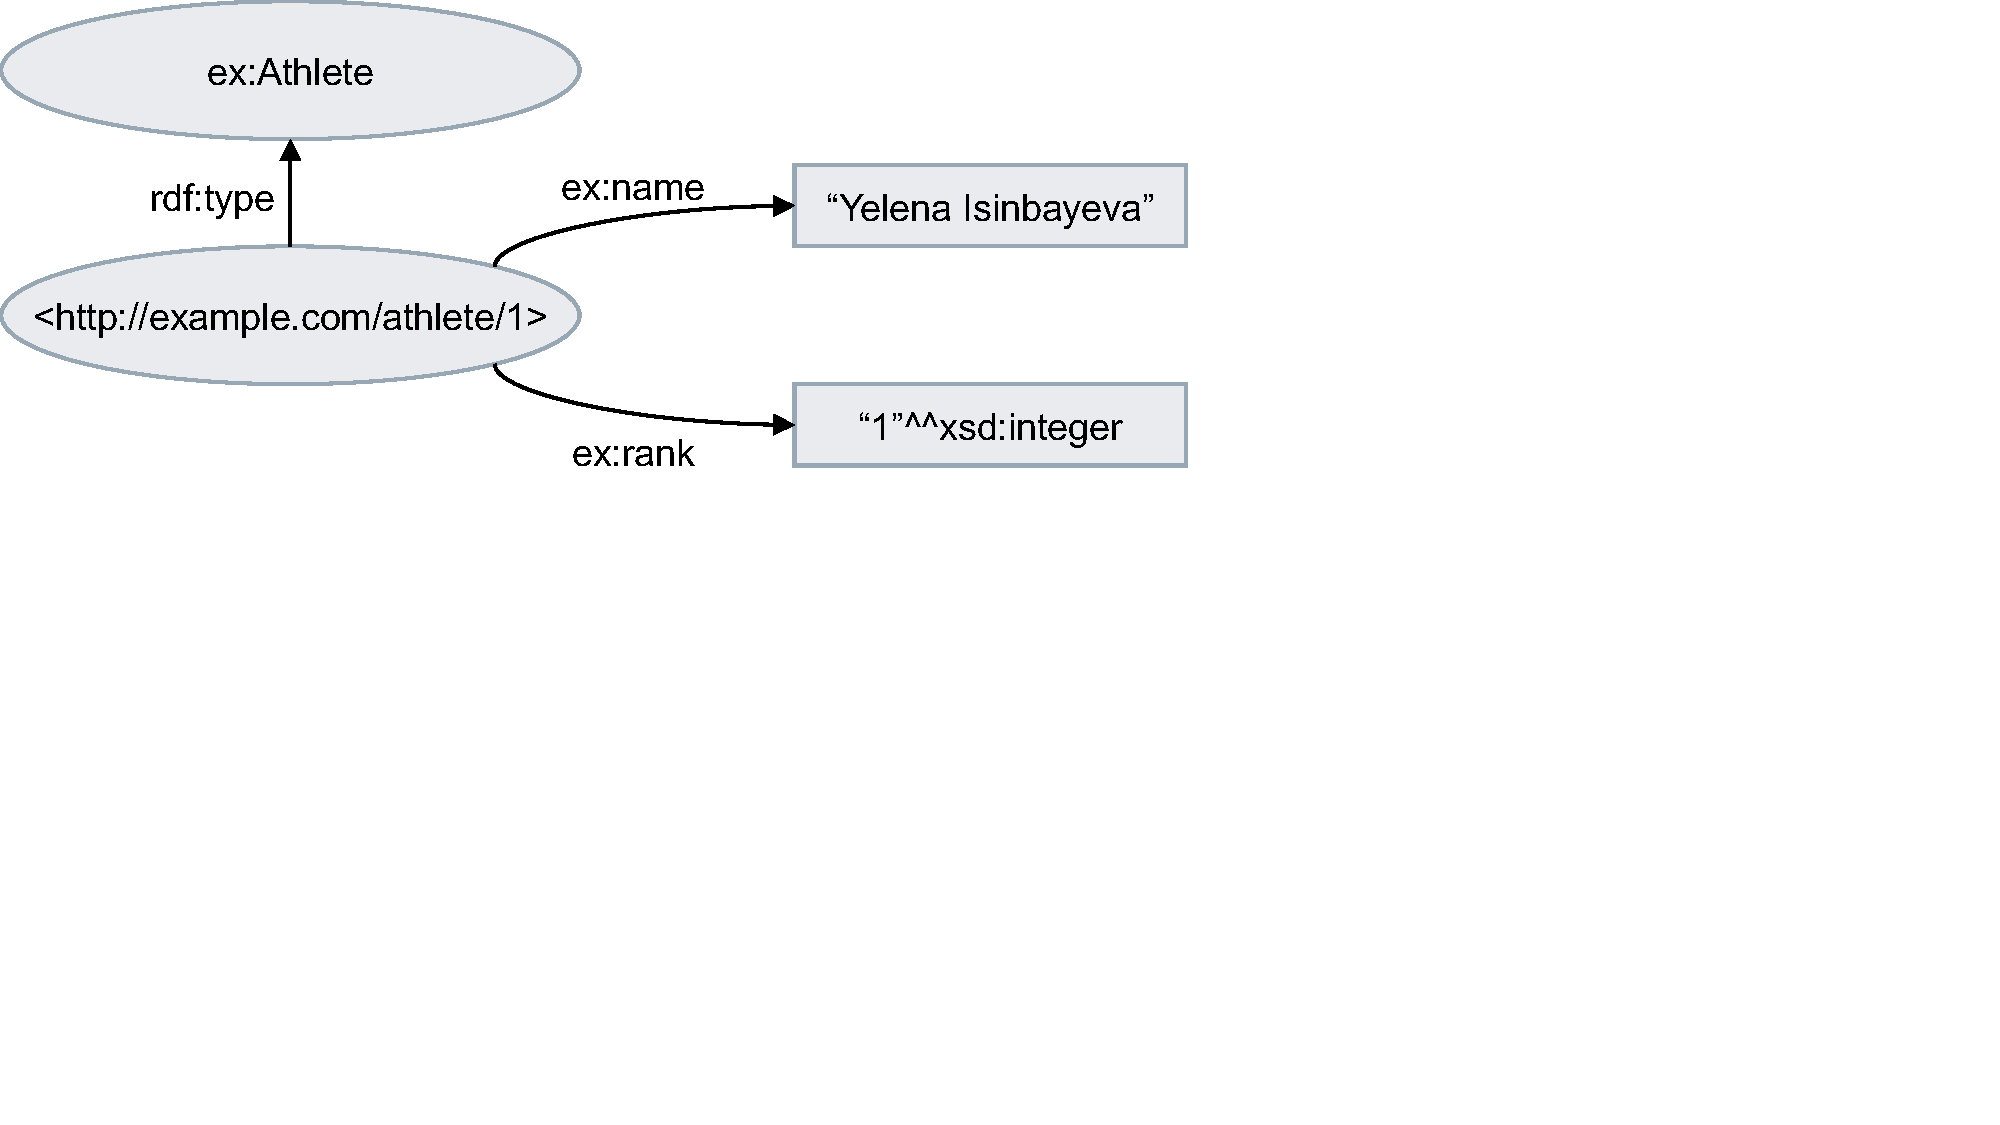
\includegraphics[width=0.6\linewidth]{figures/chp2_rdf-example.pdf}
\caption[RDG graph example]{Visual representation of the RDF graph shown in \cref{lst:chp2_rdf-example}.}
\label{fig:chp2_rdf-example}
\end{figure*}

\subsection{Statements about statements in RDF}

\ana{basic intro about what is this for and mot example about info that cannot be plainly represented in RDF. Then present all approaches used along the document: std reification, n-ary relationships, singleton properties, rdf-star, named graphs, i'd leave wikidata out of this}